\chapter{Navigation tools}
\label{chap:navtools}


This chapter discusses the requirements 
of a navigation system for a blind person 
in context of indoor and outdoor navigation. 
The popular navigation tools in use of
blind people are reviewed followed by 
some research projects which assist the 
navigation process.

%important presents reuiremneprovides an overview of some mobility 
%tools which assist the blind people during navigation. 
%The indoor navigation based on different 
%technologies such as WIFI, laser scanner etc is discussed. 
%Understanding the characteristics 
%and limitations of technologies is important to identify the 
%requirement of a vision based indoor navigation 
%system. Finally, the chapter highlights some of 
%the image based localisation works done in 
%indoor and outdoor environments. 

%------------------------------------------------------
\section{Navigation system requirements}
\label{sec:nsr}

Blind people need different functionalities from 
a navigation system. They make choices when it comes to travel and 
use different navigation tools depending upon their 
preferences.The navigation tools help the 
blind people to move safely in an environment. 
Different navigation tools are designed 
which address blind people requirements 
during the navigation. It is important to have a 
good understanding about these requirements 
before designing any navigation tool. 
Therefore, we began our research by conducting interviews 
with blind people. The interviews took place 
in Disability Information and Support Center, Otago 
University\footnote{\url{http://www.otago.ac.nz/disabilities/}}. 
The main purpose of the interview was the 
 requirement analysis i.e. figure out the 
functionalities, a blind person expects  from 
a navigation system. The requirements of a blind 
person from a navigation system 
are summarized as follows (~\citet{interview10}): 

\begin{itemize}
\item \textbf{Pedestrian Crossing:} 
The navigation system should guide the blind person
to remain in the center and to move in the right direction 
while on the pedestrian crossing. The crossing distance,
intersection street name, traffic rules etc information 
should also be communicated to increase the surroundings 
perception.

\item \textbf{Curbs Detection:}
The possible curbs or holes in the path 
should be detected and blind user should be alerted 
so that  precautionary steps can be taken 
to ensure the safety.  

\item \textbf{Sign boards:}
The system should recognize the places 
or landmarks  from sign boards. The location 
details along with the distance 
information to that landmark 
should be communicated to the user.

\item \textbf{Temporary Hazards:}
The temporary hazard signs such 
as wet floor signs, warning signs 
on a construction site etc must be detected 
and corresponding information 
should be communicated to the 
blind user. 

\item \textbf{Key destinations:}
The blind user should be guided to 
important city destinations such as hospitals, 
supermarkets, bus stops, airport etc.

\item \textbf{Speech accent:}
Navigation systems often use voice 
to communicate with its user but .
accent of the speech is sometimes 
not easy to understand. Therefore, a Braille display 
should also be available along 
with the system for further convenience.   

Braille displays are un-electro mechanical devices 
for displaying braille characters usually by means of 
raising dots through holes in a flat surface (~\citet{braille12}). 
Blind users use it to read text output.

\item \textbf{Indoor Localisation:}
Blind people want to know about 
their current indoor location in unfamiliar 
buildings and feel lost in the absence of such information. 
Therefore, a system with such functionality 
is required by the blind people. 

\item \textbf{Obstacle avoidance:}
The system should detect and alert user about 
the possible obstacles in the path to avoid the collision. 

\item \textbf{Toilets:}
The system should be able to classify the male 
and female toilets in buildings. 

\item \textbf{Scene description:}
Some sort of room description such as power socket location, 
exit doors information (opening inside/outside), 
wireless access points etc should be conveyed to the blind user. 
The location of power sockets is especially very 
important because blind people need to charge 
the carrying electronic devices. 

\item \textbf{Stairs:}
Blind people prefer lifts and the system 
should guide the blind users towards the lift. 
However, use of stairs should also be incorporated 
to deal with the emergency situations. 

\item \textbf{Guidance in the corridors:}
The system should indicate the steps 
information after which the turns are coming 
in the corridors of indoor buildings. 

\end{itemize}

Above, we have discussed the desired requirements from 
a navigation system for blind people. We realized from 
the interview that \emph{indoor localisation is one 
of the important requirement for blind people 
as they often visit unfamiliar buildings 
and have to rely on the near by people 
for the guidance.} 

It is quite hard to address all 
requirements in a single research work. 
However, these problems are addressed separately in 
different research works. Few vision based research works 
addressing the mentioned requirements are mentioned below:-

\begin{itemize}
\item (~\citet{coughlan07}) developed a 
navigation tool based on vision algorithm 
to detect the curbs and holes 
for blind wheelchair users. 
The disparity map is retrieved from stereo images 
followed by the generation of an edge map. 
On edge map, each pixel is checked for 
an appropriate depth leading to detection 
of possible curbs or holes and user is
alerted.

\item (~\citet{beno10}) presented a visual saliency 
based assistance system to point 
out areas of interest in a scene that 
present either particular interest or 
potential threat . 
The areas of interest refer to those 
objects that attract the visual attention 
of a human being. 

The system makes uses of a stereoscopic camera, 
a laptop and standard  headphones. 
The user first defines an objective such as 
find an object, find a door etc. Depending upon 
the objective, system computes the 
specific feature maps (colors, orientations, 
edges etc) and corresponding 
Conspicuity maps which lead to focuses 
of attention (FoA).  A conspicuity map 
contains information about regions of an 
image that differ from their neighborhood. 
When FoA is seen over number of frames, 
the user is informed with the global position of object or 
obstacle through a voice message.

\item \emph{See Color} is a navigation tool designed 
to provide the environment information to its 
blind users by transforming the colored pixels 
into musical instrument sounds (~\citet{beno09}. 
See ColOr encodes the colored pixels from frontal 
images by spatialised musical instrument sounds in order to represent
the color and location of visual entities in their environment. 
The basic idea is to represent a pixel as a directional sound
source with depth estimated by stereo-vision. Finally, each emitted sound is
assigned to a musical instrument, depending on the color of the pixel.
The experiments demonstrated that blind users can 
perform simple tasks like following a colored line, finding a colored 
object etc with this approach. 

\item  (~\citet{ezaki04}) presented a system capable 
of detecting the text from natural scenes 
to assist the visually impaired people. 
The system uses PDA, CCD-camera (placed on user shoulder) 
and the voice synthesizer. The image is captured and system 
automatically searches for text areas with smaller characters 
whilst person walks. In case of text area detection, the camera zooms 
to obtain a more detailed image and characters are 
recognized. The characters are then read out by the synthesizer 
to the visually impaired person. 

The morphology and binarization operations 
are used to detect the text regions from the 
captured image in the start. After zooming in, 
methods either based on edge or color are used 
to extract the larger characters in form of connected 
components. Finally, certain rules such as size, spacing 
between the characters etc are used to filter out the wrong 
text areas and come up with correct ones. The extracted 
characters then can be read out to visually impaired people. 
\end{itemize}


%------------------------------------------------
\section{Assistive Technology}
\label{sec:technology}
It include assistive, adaptive and rehabilitative devices 
for people with disabilities. The assistive technology is provided 
by the navigation tools and is used by the individuals 
with disabilities to perform functions that might 
otherwise be difficult or impossible.
The assistive technology has made possible for 
blind people to get the education and then pursue a 
career because of the use of computers and other devices.
The assistive technology for blind people include 
(1) programs that run on the computers 
to speak the text on the screen, 
and (2) stand alone products designed to 
serve as a navigation or mobility tool including applications 
designed for smartphones, personal digital assistants 
(PDAs). There are two types of navigation tools :

\begin{itemize}
\item \textbf{Primary tools:}
These tools aim to provide a safe navigation 
and are needed by blind people 
while navigating in an environment. 

\item \textbf{Secondary tools:}
These tools only increase the surroundings 
perception and must be used with some primary 
tool.

\end{itemize}

285 million people in the world are visually impaired 
and about 14\% of them are blind. 
The majority of the world's visually impaired people 
(90\%) lives in developing countries. 
The last few years have therefore seen the developments 
of different navigation tools in developing countries 
to help the blind people. At any given time, 
blind person can travel using a human guide, 
which involves holding onto someone's arm or they 
use some navigation tools.
This section lists some of the popular 
navigation tools 
used by the blind people in daily life.

\subsection{White Cane}
\label{sec:whitecane}

It serves as a primary tool and is 
commonly used by blind people. 
White canes are less expensive and offer a 
cheaper solution.
Blind people have been using a stick, 
cane or shepherd's staff as an 
assistant tool for independent travel since centuries. 
It was not until last century, the importance 
of the white cane as a symbol was 
realized. The white cane was used as a symbol for the first 
time by James Briggs in 1921 in order to alert passing 
motorists that he is a blind traveler. After World War II, 
the number of returning blinded veterans 
were quite high which further shed light on the 
significance of white canes. Different types of 
white canes have been developed so far
to address different requirements (Appendix A). 
With time, the awareness of white cane has 
increased and now it serves a dual role of both a travel 
tool and symbol identifying the user as a blind traveler
in our society (~\citet{cane1,cane2}). 
White cane is really useful for blind people 
to center themselves while walking in the corridors, 
detecting the obstacles on the way etc as 
shown in Figure \ref{fig:cane}. However the 
tactile information within the reach of the cane is only available. 
The situations that require route planning in unfamiliar environments 
will be difficult rather impossible with only white cane. 


\begin{figure}[h!]
\centering{} 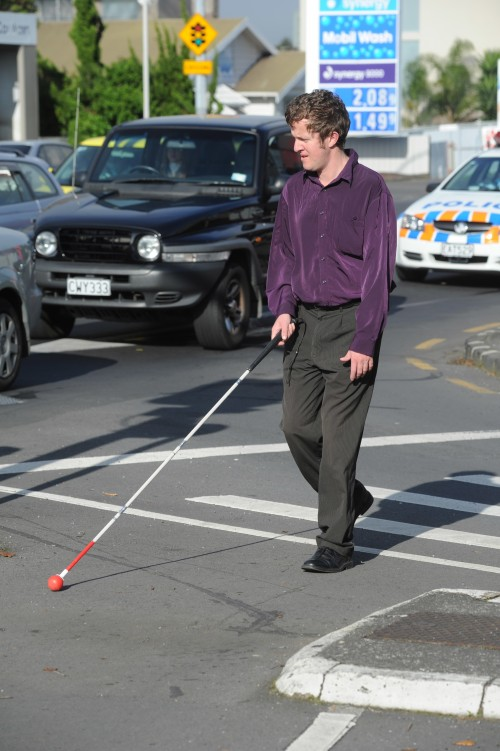
\includegraphics[width=0.3\textwidth]{Images/whitecane.png}
\caption{\label{fig:cane} Blind person on the pedestrian crossing carrying a white cane.}
\label{fig:dog}
\small (Source :\url{http://www.rnzfb.org.nz})
\end{figure}

\subsection{Guide Dogs}
\label{sec:guidedog}

The guide dog is a useful primary 
navigation tool for blind people. 
The guide dogs are trained to 
guide their users around hazards, negotiate traffic, 
locate common destinations 
such as the supermarket, post shop, travel on buses etc
(~\citet{dog1}).  
However, guide dogs are not capable of 
guiding the people in unknown environments 
especially in buildings. 
The blind user therefore does the directing, 
based upon skills acquired through 
previous mobility training. 


The first guide dog training school was established in 
Germany during World War I, to enhance the mobility of 
returning blinded veterans.
Later years have seen the establishments of such 
schools all over the world such as Australia, New Zealand, England etc.
There are about 240 working guide dogs in 
New Zealand (~\citet{dog2}).

The main problem with the guide dog is the 
associated cost which goes beyond 
US\$ 42,000 (~\citet{dog3}). 
This cost includes training the dog and 
providing instructions to the guide dog user. 
Blind people organizations use donations 
to prepare guide dogs and provide to blind people 
for free which limits the availability of guide dogs. 
Due to this reason, white canes are alternatives 
for reasons of price and in case of some people 
with allergies. Today, most blind people still use canes 
at least sometimes, some prefer guide dogs only 
and some use both as shown in Figure \ref{fig:dog}.   





\begin{figure}[h!]
\centering{} 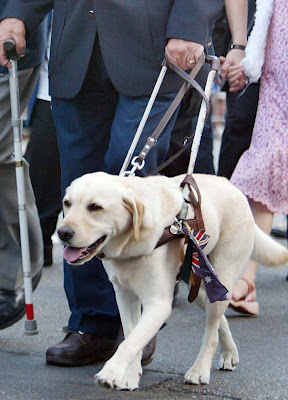
\includegraphics[width=0.2\textwidth]{Images/guidedog.jpg}
\caption{\label{fig:guidedog} Blind person along with a guide dog 
and holding a white cane.}
\label{fig:dog}
\small (Source :\url{http://theexistenceofournaturalenvironment.blogspot.co.nz/})
\end{figure}


\subsection{Miniguide}
\label{sec:miniguide}

Miniguide is a secondary travel aid 
to detect obstacles on the way. 
It is light weight, hand held and 
pocket size device as shown in Figure \ref{fig:miniguide}.
The device uses ultrasonic echo-location 
to detect the obstacles or objects whilst blind person 
navigates. The aid vibrates to indicate the distance to objects 
i.e. a faster vibration means that the object is nearby. 
The device can be adjusted to detect obstacles within different 
distance ranges e.g. 1 meter, 2 meter etc. However, 
only large objects can be detected at 
4 meters or beyond, for example, fences, walls.


\begin{figure}[h!]
\centering{} 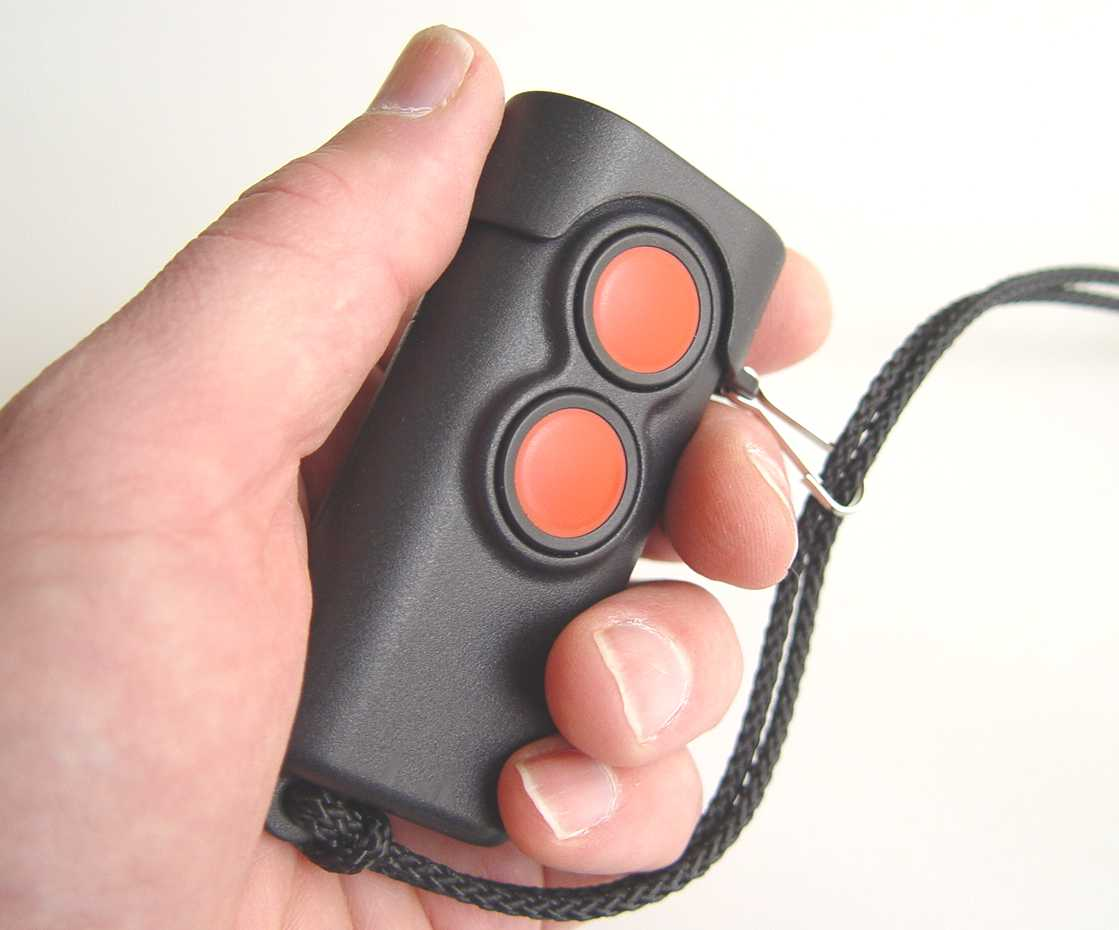
\includegraphics[width=0.2\textwidth]{Images/miniguide.jpg}
\caption{\label{fig:miniguide} Person holding a miniguide.}
\small (Source :\url{http://www.gdp-research.com.au})
\end{figure}

Miniguide has assisted blind people in 
many ways such as avoiding obstacles, 
detecting overhanging obstacles 
(tree branches), locating door ways etc. 
With all these merits, it cannot detect drop offs and 
the cost of miniguide is up to US\$ 400 which 
make sit hard for blind people to afford it (~\citet{miniguide}).

\subsection{Soundpost}
\label{sec:soundpost}

Soundpost is a primary navigation tool. It is 
basically an orientation device and uses 
infrared technology to guide the blind person 
to move accurately from one landmark to the 
other (~\citet{povidi}). It allows 
a blind person to cross up to 
30 meters of an open space. Soundpost uses multiple base stations for generating 
signals and blind person carries a hand held transmitter to 
receive the signals as shown in Figure \ref{fig:soundpost}.
The transmitter starts vibrating once it comes within range 
of a base station and keeps on vibrating until 
you move towards the landmark. 
The transmitter can also generate 
a voice message indicating the landmark information. 


\begin{figure}[h!]
\centering{} 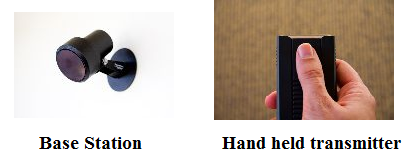
\includegraphics[width=0.5\textwidth]{Images/soundpost.png}
\caption{\label{fig:soundpost} Soundpost device.}
\small (Source :\url{http://www.povidi.com/SoundPost.html)}
\end{figure}

  
A small independent trial is undertaken at the 
University of Canterbury, New Zealand to assess its 
utility for a blind citizen. It has been preferred by both 
guide dogs and white cane users as it further assists 
the navigation in any environment. However it suffers 
from following problems which limit its applicability:-

\begin{itemize}
\item The infrared signal is often broken 
which pose problem during the navigation.

\item It's hard to estimate the 
movement direction towards the landmark 
once the vibration starts.

\item The voice messages are limited.

\item It costs about US\$500 which includes 
the transmitter and two base stations.
\end{itemize}


\subsection{Loadstone GPS}
\label{sec:loadstone}

Loadstone GPS is a free open source software 
for satellite navigation for blind users (~\citet{loadstone}). 
The software currently runs on different 
Nokia devices and requires a GPS receiver.
This project was initiated by Monty Lilburn and 
Shawn Kirkpatrick back in 2004 who are 
themselves blind. The whole program is under the 
General Public License (GPL) and is financed 
entirely by the private developers and by the donations. 
It was made public in 2006 and has been 
a success since then.

The maps consist of way points imported from 
the common map data bases. In some 
cities, rural regions etc no 
exact map data is available in 
common map databases. In such scenarios, 
the software provides users an option to 
create and store their own way points 
for navigation and share it with others. 
There is also a website which allows users 
to share there custom points with each other
and points can then be easily added to the map. 



This application is useful to search for specific locations 
in a given area. However, it lacks some of the 
basic features such as automatic download of maps 
and a route planner. Still tool is very accessible and 
useful when travelling in an area.
\subsection{Research Projects}
\label{sec:research}

In the above sections, we discussed some 
commercial products which provide mobility aid 
to the blind people. A lot of research 
has been carried out in the last few years 
to propose the reliable navigation tools. 
Some of the well known research projects 
which use computer vision and other 
technologies to aid the blind 
user mobility are discussed in the 
following sections. 

\subsubsection{Drishti}

Drishti is a navigation system capable 
of guiding and helping the blind people 
to travel safely both in indoor and outdoor environments (~\cite{ran04}). 
It uses a precise position measurement system, a wireless 
connection, a wearable computer, and a vocal communication interface. 
For outdoor, it uses differential GPS as its location system
to keep the users as close as possible to the 
central line of sidewalks of campus and downtown areas. 
The user can switch the system mode from an 
outdoor to an indoor environment with a simple vocal command. 
An ultrasound positioning system is used to 
provide precise indoor location measurements 
with an accuracy of 22 cm. The user gets 
alerts in the form of vocal prompts to avoid 
the possible obstacles. 
It performs dynamic routing and rerouting to provide 
its blind users with an optimal route for navigation. 
A step-by-step walking guidance is provided for 
navigation in environments. The proposed system is 
good but it is not easy to use as blind person 
have to carry a number of devices.



\subsubsection{Crosswatch}
(~\cite{james08}) presented Crosswatch,
a real time mobile application 
to detect the zebra crossings in outdoor environments. 
At the proposed time, this was the first 
portable system capable of providing 
the real time orientation information 
at urban traffic intersections. 
The system first extracts the straight line segments 
as features from the mobile image. A factor graph model 
is then used to group the features into figure and ground, 
representing crosswalk and background respectively. 
The detection of enough features having sufficient length 
indicates the detection of a cross walk 
and a brief audio tone is sounded for frames 
in which a crosswalk is detected. 
Nokia N95 mobile phone is used in experiments 
which can process approximately three frames per second.
The application is tested with blind subjects to test the usability 
and the subjects answered correctly whether a zebra crosswalk 
is present or absent at all used intersections. 



 (~\cite{james10}) further extended Crosswatch 
to incorporate the detection of 
walk lights on the pedestrian crossings.
Crosswatch is now capable to alert the user 
once the green walk light is illuminated at the intersections. 
Corsswatch is robust, easy to use and performs well in urban 
intersections in the United States.


\subsubsection{Electro Neural Vision System (ENVS)}
(\citet{meers05}) presented ENVS, a system capable 
to avoid obstacles, perceive landmarks 
and assist in navigation via visual sensors, 
GPS and electro-tactile stimulation. 
ENVS first extracts the depth information from the
environment via disparity map 
obtained from the head mounted stereo cameras as shown in 
Figure \ref{fig:envs}. 
This range data is then delivered 
to the fingers via electro-neural stimulation to indicate 
the range of objects being viewed by the cameras to the 
user. To perceive the location of obstacles and the 3D structure 
of the environment, user imagines that the hands are held 
in the direction viewed by the cameras, with fingers 
extended and the amount of stimulation 
felt by each finger indicates 
the range of objects in the pointed direction. 

\begin{figure}[h!]
\centering{} 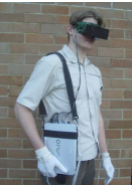
\includegraphics[width=0.3\textwidth]{Images/envs.png}
\caption{\label{fig:envs} The Electro- Neural Vision System.}
\small{Source: (~\citet{meers05})}
\end{figure}

In order to perceive landmarks, 
ENVS uses a GPS, a digital compass and a database of landmarks. 
The relative location of significant 
landmarks is determined (using GPS and stored GPS 
coordinates) and delivered to the fingers via encoded pulses 
when the landmarks are in the field of view. 
The system does quite well in conveying the 
3D structure of the environment to the blind people. 
The experimental results indicate that ENVS 
enables the user to achieve localization, 
obstacle avoidance and navigation without using the eyes. 
However, it is not easy to use because 
blind user needs to carry a laptop and wear gloves 
for ENVS.


\section{Summary}
The purpose of this chapter was to provide a 
overview of navigation system requirements 
and highlight the importance of indoor localisation 
for blind people. Some popular navigation tools along 
with the research projects which aid 
the navigation process are discussed. 
In the next chapter, we discuss the navigation
systems which mainly use computer vision 
techniques such as features, topological maps, 
scene localisation to provide navigation in indoor environments.  
Research works addressing the scene localisation 
problem in indoor and outdoor environments
are presented towards the end in the next chapter.





%
%\begin{enumerate}
%\item \textbf{Pedestrian crossing guidance} 
%\item \textbf{Curbs/Holes identification on the track}
%\item \textbf{Sign boards classification}
%\item \textbf{Temporary hazards identification}
%\item \textbf{Key destinations identification}
%\item \textbf{Voice accent understanding}
%\item \textbf{Location recognition}
%\item \textbf{Obstacle avoidance}
%\item \textbf{Toilets gender categorization}
%\item \textbf{Scene description}
%\item \textbf{Stairs guidance}
%\item \textbf{Guidance in corridors}
%\end{enumerate} 

%
%\section{Indoor Navigation Systems}
%Simultaneous localization and mapping (SLAM) is a 
%technique used by robots and autonomous vehicles 
%to build up a map within an unknown environment (without a priori knowledge), or to update a map within a known environment (with a priori knowledge from a given map), while at the same time keeping track of their current location.
%
%Indoor navigation systems are based on different technologies 
%such as WIFI, laser range etc. Each technology used for 
%indoor navigation system has its pros and cons. Some commonly used 
%technologies for indoor navigation system are as follows:-
%
%\subsection{Using Laser Scanner} 
%In indoor, the localization using laser range 
%finder has been used a lot. However these 
%methods provide a 2D map of the environment. 
%
%The navigation system these days are based on different technologies.
%Every technology has it pros and cons.
%
%\subsection{With WIFI Fingerprints}
%\subsection{With Images}
%\subsection{With Smartphones}


%\section{Visual Navigation}
%\label{sec:visualnavigation}
%
%The vision (image or videos) has become common in applications 
%such as localisation, automatic map construction, 
%autonomous navigation, path following etc in the 
%last few years. The navigation techniques based 
%on vision increase the scope of application of autonomous 
%mobility and have resulted in countless research 
%contributions for robots, autonomous ground vehicles, 
%unmanned aerial vehicles and blind people. 
%The systems that use vision for navigation can be 
%divided into two main categories:-
%
%\subsection{Map based systems}
%\label{sec:mapbasedsystem}
%
%This include those systems that either 
%need to have some representation of the environment 
%before the start of navigation process. 
%There are three systems 
%mainly (1) systems that need a complete map 
%of the environment before hand referred as \emph{map-using}, (2) systems that explore the environment 
%and automatically build a map off line referred as \emph{map-building}, and (3) systems that perform 
%the map construction online referred as \emph{local map-based}.
%
%In \emph{map-building} approaches, precise localization is important 
%for accurate map building and is the must needed functionality. 
%In standard \emph{map-building} systems, it is assumed that localisation 
%can be computed by some other techniques. However in 
%pure localisation approaches the map is presumably 
%available and systems need to track its own position and orientation in 
%the environment continuously. If the exploration and mapping of an 
%unknown environment is done automatically online, the navigation system 
%needs to explore, map and localise itself simultaneously usually 
%referred as Simultaneous localization and mapping (SLAM). 
%Recently, cameras have been used as the sole sensor
%yielding visual SLAM (~\citet{chen07, davison07}). In this section, 
%we discuss vision based navigation systems with a 
%that belong to one of the three mentioned categories 
%and work in indoor environment.
%
%Sim \emph{et al.} presented a system that is capable of
%mapping a large, complex visual environment in real time using 
%a pair of stereo cameras (~\citet{sim06}). 
%The system explores, navigates autonomously and
%generates a hybrid map representation that facilitates the 
%accurate localization (using visual landmarks) and safe
%navigation (using occupancy grids). The landmarks are 
%detected in images using the SIFT features (~\citet{lowe04}), 
%matched using best bin search and are stored. 
%This is followed by an occupancy representation 
%to obtain a reliable spatial representation 
%of the world to ensure real time safe navigation. 
%They used an Activmedia Powerbot robot 
%with a stereo head. The robot explored and 
%did well in a laboratory environment
%consisting of two rooms of total size approximately
%19m by 16.5m.
%
%A topological map is a graph based representation 
%of the environment where each node corresponds to a 
%zone of the environment and can be associated with 
%action such as turning, crossing a door etc.
%Gaspar \emph{et al.} used omnidirectional camera 
%to create a topological map of the indoor structured 
%environment during a training phase (`\citet{gaspar00}).
%The insect vision based capability was emulated allowing the system to advance 
%along corridors, recognize the ends, turn into correct directions 
%etc. Each node is recognizable with landmarks and covers the movement 
%between the two nodes for instance two doors joined by a corridor.
%
%Kidono \emph{at al.} developed a system which needs human guided 
%pre-training phase (~\citet{kidono02}). 
%A human guides the robot through an environment 
%and during this guided route, the robot records images 
%with a stereo camera. The recorded images are used 
%to construct a 3D map on line incrementally 
%frame by frame. Once the map is built, the robot can 
%repeat the same route from the starting point to the 
%goal point, tracking features and computing 
%the closes safe path. The robot was
%navigated in an indoor environment and performed well.
%
%
%
%Anther important application of map building navigation systems 
%are the museum guiding robots. These robots need to be autonomous 
%to recognize people, guide them through different environments 
%and also avoid obstacles. Thrun \emph{et al.} developed a robot 
%MINERVA that uses two cameras combined with a laser sensor 
%to build map of the environment for the navigation process (~\citet{thrun99}).
%MINERVA uses laser scans, camera images and odometry 
%readings to build the occupancy and texture maps 
%via joy-sticking the robot through its 
%environment during training phase. Texture maps
%of the ceilings are generated using image mosaics 
%to handle the crowd with in the museum.
%The robot remained operational for two weeks 
%Smithsonian’s National Museum of American History 
%and successfully interacted with thousands of people.
%Shen \emph{et al.} proposed ATLAS, a museum 
%guiding robot that combines topological map building 
%image matching algorithms for localisation (~\citet{shen06}). 
%The robot is designed to detect the nearby visitors nearby 
%and interact with them via voice and a touching screen. 
%Moreover, system also incorporates a human face detection 
%algorithm to actively approach to new visitors.
%
%The approaches discussed so far are based on global 
%description of the environment which can be either obtained
%automatically or by a human guided stage but before the start 
%of navigation. Since the early nineties, some 
%authors have developed the navigation systems 
%which support on line construction of a local 
%occupancy grid. The local grid refers to the portion of 
%the environment surrounding the robot and grid size is
%determined by the camera field of view. This local information 
%is used for a subsequent map construction frame by frame 
%for on line safe navigation. Gartshore \emph{et al.}
%presented a system capable of building maps from online images 
%captured by a single camera.  The systems computes the 
%probabilities of finding the objects at every location. 
%The algorithm detects the object boundaries using edge and 
%corner detector. Detected features are back 
%projected from the 2D image plane considering all the potential locations 
%at any depth. The system computes the position using odometry 
%data combined with feature extraction process. Color or gradient 
%from edges and features from past images 
%help to increase the confidence of the object presence 
%in a certain location. The experiments were conducted 
%in indoor environments and robot moved 100mm between consecutive images.
%
%In the recent years, visual sonar is also used 
%for the navigation purposes. It uses range data and depth measurements 
%for navigation purposes in an analogous way to 
%ultrasound sensors. Martin used the same idea 
%to compute depth from single camera images of indoor 
%environments (~\citet{martin06}).
% The genetic programming is used to 
%discover the best algorithm to detect the ground boundaries 
%in a training phase. These algorithms then use obstacle 
%avoidance strategies initially developed for sonar.
%The algorithms are designed to be a 
%replacement for sonar, returning the location of
%the nearest obstacle in a given direction. The three 
%indoor data sets were used with a total of 
%images from four different hall ways.
%
%\subsection{Mapless systems}
%These refer to those techniques which do not need 
%any knowledge of the environment but they navigate 
%as they perceive the environment. These techniques 
%often grab video frames to produce enough information 
%about the unknown environment and navigate through it 
%safely. 
%
%Optical flow is one of the technique commonly used 
%for mapless systems. It can be defined as apparent motion 
%of features in a sequence of images i.e. video frames.
%Taludker \emph{et al.} (~\citet{talukder04}) 
%presented optical flow based 
%solution to detect the dynamic objects in the camera field of view.
%The system assumes that dynamic objects create discontinuity 
%in optical flow orientation and changes in magnitude with respect to the 
%background pixels optical flow direction and magnitude. The system 
%is tested using a single camera and later enhance with a stereo camera.
%
%Green \emph{et al.}  (~\citet{green03}) 
%described the design of a robot that can fly in 
%the buildings controlled by an insect inspired optical flow based system. 
%The relevance of insect based navigation strategy in an optical flow 
%based navigation was emphasized in the work.
%
%
%Appearance based navigation strategy record images or 
%prominent features of the environment as model templates. The 
%models are basically labeled with a certain location information. During
%navigation stage, the robot matches on line image with stored images. 
%The main problems with such approaches are (1) how to create environment 
%representation (2) performing the online matching criteria. 
%In such techniques, loop closure i.e. detection of previously 
%recorded images plays an important part during the navigation 
%phase. 
%
%Zhou \emph{et al.} (~\citet{zhou03}) 
%utilized histograms based on color, gradient, 
%edge density and texture to describe the appearance 
%of trained images. The recognition during online stage is 
%performed by matching the histogram of query image with the 
%stored templates. 
%
%Remazeilles \emph{et al.} (~\citet{remazeilles04}) used an appearance based navigation 
%system. The system uses an image data base which is a set of views 
%built off line representing the whole navigable environment.
%Once navigation mission is defined, an image sequence corresponding to 
%what robot should see during the motion is extracted from the data base.
%The robot motion is the result of online detection and matching 
%process between the models included in the sequence and 
%perceived scenes.To navigate, the robot tracks recognizable previously cataloged 
%features.
%
%Fraundorfer \emph{et al.} (~\citet{ fraundorfer})proposed vision based localisation and mapping 
%for robot navigation. The environment is represented as a linked 
%collection of way point images. The collection is built online while 
%robot is exploring the environment.  Links are created between the 
%sequential images and are inserted by image matching. 
%An efficient image matching scheme allows real time mapping and global 
%localsation. 
%
%Booji \emph{et al.} (~\citet{booji}) 
%proposed navigation via image based topological map. 
%The robot is driven through the environment and keeps on 
%taking the pictures. The system uses epipolar constraints 
%based on SIFT features to match the images. By conputing the 
%similarities between these images a topological map 
%in form of in form of an appearance graph is created.Navigation on 
%this graph involves heading from one node to the other.
%
%Se \emph{et al.} (~\citet{se01}) proposed a vision based localisation and mapping 
%algorithm which uses scale invariant image features as landmarks in unmodified 
%dynamic environments. The 3D landmarks are localised and robot 
%ego-motion is estimated by matching them 
%taking into account the feature viewpoint extraction.
%
%Feature tracking navigation systems tracks features 
%in consective frames to perform the navigation. 
%Pears and Liang \emph{Et al.} (~\citet{liang02}) 
%use hoographies to track ground plane corners 
%in indoor buildings.  The same authors extended their 
%work by using homographies to calculate the height of 
%tracked features or obstacles above the ground plane during the navigation. 
%
%During robot driving throught the environment, SIFT based methods extract 
%the important features from the environment which 
%serve as landmarks to be tracked for navigation, global 
%localisation and robust vision based SLAM performance 
%(~\citet{se02, se05}).
%%\begin{itemize}
%%\item \textbf{Map based navigation:} 
%%These systems require a map of the environment 
%%for the navigation. It also includes those systems that can explore the environment 
%%and build the map by themselves. However 
%%the environment needs to be explored first 
%%and its representation is stored before the start of navigation.
%%Therefore systems in this category will start 
%%navigation if and only the environment map 
%%is available.
%%
%%\item \textbf{Mapless navigation:}
%%It includes all navigation approaches that do not 
%%require any knowledge of the environment for navigation
%%run. Navigation is performed on the basis of elements 
%%observed in the environment such as walls, features,
%%doors, desks, etc. 
%%
%%\end{itemize}
%%
%%In the last few years, lot of progress is observed in context 
%%of visual navigation. The older techniques have been refined 
%%and lot of new techniques are also presented 
%%which have led to a more accurate and 
%%efficient navigation systems. We review some of the 
%%visual navigation approaches used for map based and 
%%mapless navigation in the following sections. 
%%
%%
%%\subsection{Map based systems}
%%This category includes systems that need a complete map 
%%of the environment before the start of navigation.
%%Other systems in this category are able to 
%%explore the environment and 
%%automatically build a map. However the navigation 
%%phase will start only once the map is built. 
%%The map information can be directly 
%%used for navigation or it can be
%%post-processed to improve the map accuracy
%%to achieve a more precise localization. 
%%
%% 
%%\section{Visual Indoor Navigation}
%%\begin{enumerate}
%%\item Map based navigation
%%\begin{enumerate}
%%\item Topological maps
%%\item Local maps
%%\end{enumerate}
%%
%%\item Map less navigation
%%\begin{enumerate}
%%\item Optical Flow
%%\item Appearance based navigation
%%\item Feature based navigation
%%\end{enumerate}
%%\end{enumerate}
%
%
%%\section{Simultaneous Localisation and Mapping (SLAM)}
%%A brief discussion about SLAM.
%%\subsection{Visual SLAM}
%%Discussion about SLAM based on images.
%%I will mention some of the research works 
%%based on Visual SLAM for robotics.
%
%\subsubsection{Loop Closure}
%Discuss the importance 
%of loop closure i.e. identification of the place 
%which has been already visited.
%
%
%
%\section{Image based localization}
%I will state that our indoor location recognition is 
%also based on image based localisation.
%We are doing a 2D image base matching.
%I will discuss some research works briefly 
%which have done localisation in indoor environments
%using different techniques based on 2D images.


